% !TeX root = paper.tex
\documentclass[a4paper,12pt]{article}

% Packages
\usepackage[utf8]{inputenc}     
\usepackage{amsmath, amssymb} 
\usepackage{graphicx}          
\usepackage{geometry}           
\usepackage[numbers]{natbib}            
\usepackage{hyperref}          
\usepackage{subcaption}         
% Page layout
\geometry{margin=1in}          

% Title section
\title{TIM: Tree Imaging Machine}
\author{Your Name}
\date{\today}




\begin{document}

\maketitle

\begin{abstract}
The Tree Imaging Machine (TIM) is a do-it-yourself scanning tool made to digitize tree cookies and cores. TIM takes partially overlapping microscopic images of samples and stitches the individual images together to form 
a mosaic. These scans can produce multiple gigabyte stitched images which can be zoomed in to see distinct features on the scale of 0.01mm. With scans of up to 21,140 DPI, TIM produces one of the highest resolution images among similar tools.
We designed TIM to have a large working plane to allow the digitization of individual cores over 50cm and to allow the operator to set a batch of samples to be digitized without intervention. 
All of the 3D printed parts are available for download on the NIH 3D printing repository and the software is 
open source. Instructions to recreate this tool can be found on the code repository. 
\end{abstract}

\section{Introduction}
The study of tree rings has proven useful across multiple fields, proving to be a reliable subject for reconstructing past climates of regional and local environments, as well as a mechanism to understand tree growth response \citep{fritts_dendroclimatology_1971} \citep{williams_using_2010} \citep{guibal_dendrochronology_2021} \citep{sheppard_dendroclimatology_2010}.
To obtain these data from the tree rings, it is necessary to measure tree rings from a tree cookie or core. The first high precision tool for this purpose was a stage micrometer, involving a trained technician to incrementally shift a tree core under the objective of a microscope - informing a computer when a new ring is encountered \citep{robinson_microcomputer_nodate}.
While this method has very high precision, the data is only as accurate as the experience and knowledge of the technician at the time of recording \citep{levanic_atrics_2007}.
The desire to remove repetition of errors in sampling and sampling bias across to individual technicians led researchers to an alternative - image analysis. 

The first step in measuring tree ring width from images requires the digitization of the sample from one of two major methods.  
The original technique was as a flatbed scanner which can digitize the entire sample at once \citep{guay_new_1992}. 
With a top of the line scanner, like the Epson Perfection V850 Pro, it's possible to scan at maximum resolutions of 4800 dpi and scan an area of up to 8.5" x 11.7".
Analysis which relies on higher resolution larger samples require a different digitization approach. 

The second digitization model was introduced with ATRICS \citep{levanic_atrics_2007}. 
Rather than scanning a whole sample at once, a high resolution camera takes multiple images across the surface of the sample and uses image stitching software techniques to combine them into one ultra high resolution image \citep{muhlich_stitching_2022}.
Stitching multiple images into one mosaic has been applied in other fields such as mineralogy and cellular biology \citep{ro_image_2021,mohammadi_fast_2024}. 
This method requires either the camera objective to move relative to the sample, or the sample move underneath a stationary camera. 
For ATRICS and a more modern do-it-yourself alternative, CaptuRING, the sample is moved relative to the camera \citep{garcia-hidalgo_capturing_2022}. 
Gigapixel takes a different approach by moving the camera relative to the sample, allowing for multiple samples to be recorded in sequence \citep{griffin_gigapixel_2021}. 
While these machines can all digitize cores, none have been shown to digitize cookies.

TIM was made to combine the defining features of the previously mentioned machines into one while making the project open-source and open-hardware. 
We designed TIM to digitize both cookies and cores, increase the maximum sample length, perform image stitching without operator intervention, all while minimizing cost. 
Successful functionality of this system is dependent on the major steps in tree cookie and core digitization to be automated. 
The only specialized piece of equipment needed to build TIM is a 3D printer, but the parts can be readily ordered through 3D print shops if preferred.
Excluding 3D printed parts, the total cost of the machine is approximately \$2,200 USD compared to the \$70,000 USD of the Gigapixel \citep{griffin_gigapixel_2021}.
The total cost of the machine is almost comparable in price or less to many professional camera and macro lens combinations.
Additional savings can also be had when factoring in the cost of a professional stitching software license such as PTGui. 

\section{Methods}

\subsection{System Overview} % this is so dry fix later

TIM can be thought of as a combination of multiple subsystems: the camera, computer, and gantry machine. 
Cartesian movement in the X, Y and Z directions is a result of two machine kits and a motor controller from OpenBuilds - the ACRO 1010, the NEMA 17 lead screw linear actuator, and the X32 Motor Controller running GRBL firmware. 
Building on top of kits allowed for quick assembly with sound instructions and saved development time. 
To fit on the build plates of the ACRO system, we made an adapter to connect the linear actuator to the X and Y axis, thus creating motion in the Z axis.
On the linear actuator's build plate, adapters were made to hold a 12MP Raspberry Pi HQ Camera equipped with a SEEED studio microscope lens connected to an NVIDIA Jetson Orin Nano (Jetson) through a CSI cable.
By choosing this combination, we were able to reduce the weight and cost of the camera significantly - trickling the budget into an efficient computer which can handle intensive image processing. 
The Jetson is a powerful edge computer which drives a computer monitor for a GUI, sends commands to the motor controller to move the machine, runs image processing calculations for automatic control, and performs calculations to stitch individual images into one mosaic. 
Despite the weight reductions, torsion on the gantry arm still resulted in a non-zero torsional deflection. A torsion correcting adapter was designed to counteract this rotation and level the lens.


\subsection{Preparing Cookies and Cores}
TIM can be used to scan both tree cookies and tree cores. Sample preparation for both are equally important but require different approaches.
The scanning surface of the cookies and cores need to be sanded with incrementally increasing sand paper grit. Our cookies were sanded using a belt sander from 60 to 400 grit and polished with 1200 grit by hand.
Sanding cores was a mix of belt sander and a small orbital sander using the same grit sequence. 

Special sanding considerations need to be taken for each sample type. 
For cookies, it is important to have the top and bottom surfaces be nearly parallel. Small differences in plane angle can be corrected using the levelling table (See Figure \ref{fig:ideal_levelling}). 
For cores, care should be taken to maximize the scanning surface. This means removing material to be coincident to the center of the cross section of the core. 
Cores also need to be aligned to be parallel to the X axis to be digitized, a squaring tool helps guarantee this. Any warping in core mounts need to be counteracted with the use of clamps. 

\subsection{Sample Digitization} % Methods
The subsystems can be best understood by following the process from sample setup through the computing process to create the stitched image. 
To achieve this with a fixed focus camera, the samples must be nearly orthogonal to the camera lens. Misalignments between the sample and lens up to 10 degrees can be corrected by using the 3D printed sample levelling table we designed (See Figure \ref{fig:ideal_levelling}).
Once the sample is level, the operator interacts with the machine through the GUI to navigate the camera to the center of the sample, and focuses the preview image to be sharp by moving in the Z axis. The height and width dimensions are then entered in the GUI
to be saved along with the detected center coordinate of the sample. This procedure can be repeated to create a queue of samples to digitize.
The height, width, identifiers, and centering of the sample is sufficient information to digitize.

\begin{figure}
    \centering
    \begin{subfigure}{.5\textwidth}
      \centering
      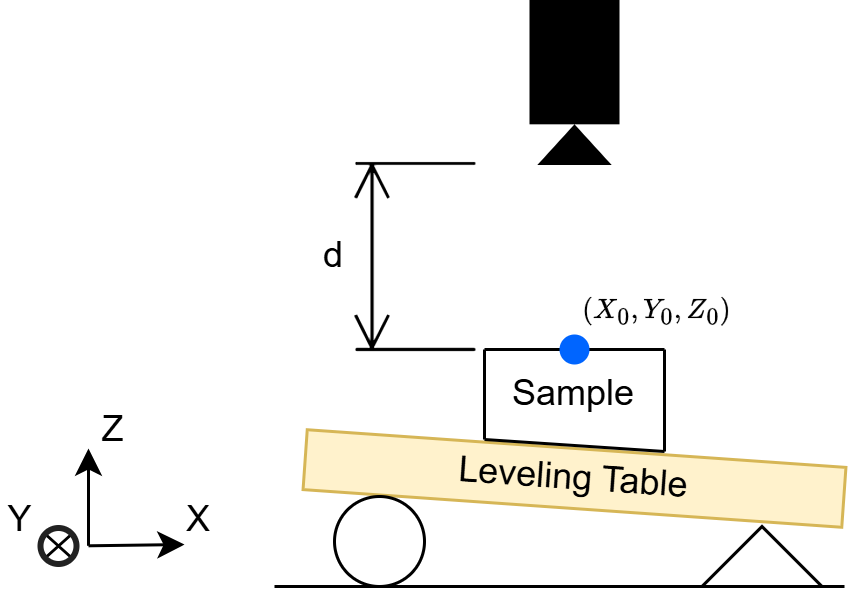
\includegraphics[height=0.5\linewidth]{../diagrams/sample_setup_ideal.png}
      \caption{Ideal sample leveling}
      \label{fig:ideal_levelling}
    \end{subfigure}%
    \begin{subfigure}{.5\textwidth}
      \centering
      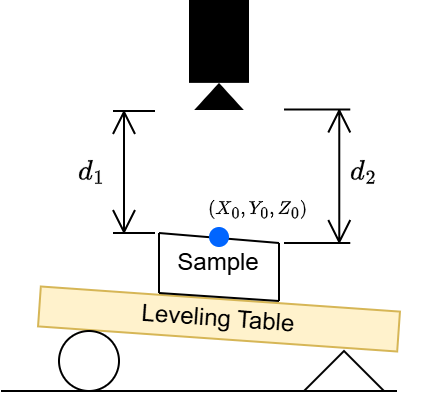
\includegraphics[height=0.5\linewidth]{../diagrams/sample_setup_realistic.png}
      \caption{Realistic sample leveling}
      \label{fig:realistic_levelling}
    \end{subfigure}
    \caption{Side view of the camera and sample on top of a leveling table. The ideal sample leveling shows a uniform distance d at all $(X,Y)$ coordinates on the sample. This is impossible to achieve in reality, the true sample leveling has a non uniform distance at unique $(X_i, Y_i)$.}
    \label{fig:sample_levelling}
\end{figure}


\subsection{Image Capturing}
In the GUI the operator indicates the height and width of the field of view in an individual image from the camera. 
This varies on the focal length of the lens, but we have kept the field of view to be 3mm x 5mm. 
Once prompted the system begins to exhaustively traverse the surface area of the sample, using the sample height and width entered by the operator.  
The goal of this traversal is to obtain in-focus images that have a region of overlap with all its neighbors - the basis of image stitching. 
Digitizing cores can be done without needing to traverse in both the X and Y axis. 
The optimal scanning path for a core is to ignore the Y axis and traverse the cores length.
Spanning the surface area of a cookie requires movement in both the X and Y axis.

By centering the design around a fixed focus camera and lens, it is necessary to implement some sense of automatic control to focus the images. 
The only way to control the focus of a fixed focus lens is by changing the lens's distance to the sample. 
And with the microscope lens, the depth of field of the image is so sensitive that a perturbation of less half of a millimeter can move an entire image out of focus.
Solving this in a time efficient manner involves two stages. 
The first stage takes advantage of the requirement to navigate and focus the camera to the center of the sample.
This allows the initial $Z_0$ value from $(X_0, Y_0, Z_0)$ to be an informed guess as to what value would have an in focus image across the entire surface. 
From the first $(X_0, Y_0)$ coordinate captured, 11 images are taken at different $Z$ values in $\boldsymbol{Z_{\text{samples}}}$. 
So long as $Z_{focused}$ is within this set, an in focus image exists.

\[
Z_{focused} \in
\boldsymbol{Z_{\text{samples}}} = 
Z_0 + 
\begin{bmatrix}
-0.5 \\
-0.4 \\
\vdots \\
0.4 \\
0.5 \\
\end{bmatrix}
% \exists 
% Z_{focused}
\] % unsure if this makes sense

Beginning at 0.5 mm above $Z_0$ and the last image finishing at 0.5 mm below $Z_0$.
To reduce motion blur in the images, the range of $\boldsymbol{Z_{\text{samples}}}$ is traversed at constant velocity and images are captured without stopping. 
The 11 images then have their normalized variance, $NV$, calculated in a separate thread to measure the image sharpness \citep{sampat_extensive_2014}.
The image with the maximum score is saved while the rest are deleted from storage.

\[
    i_{\max} = \arg\max_{i} NV(image(\boldsymbol{{Z_\text{focus}})})
\]
    
This focusing procedure works well alone when the sample alignment has a difference in height no greater than 0.5 mm, $d_1 - d_2 < 0.5 mm $ (See Figure \ref{fig:realistic_levelling}). 
% And while 1mm may sound like a small range, it is important to note that increases in time at each $(X_k, Y_k)$ are repeated $k$ times. 
Rather than adjusting this range, a greater alignment error can be managed by controlling the center of the range, $Z_{0,k}$, for $(X_k,Y_k)$. 
The likelihood of an adjacent $(X_{k+1}, Y_{k+1})$ containing an in focus image is highest when the current $i_{{\max,k}}$ is at the middle index of $\boldsymbol{Z_{samples}}$. 
A PID control algorithm with a process variable of $i_{max}$ and control variable of $Z_{0,k}$ allows a negative feedback loop to improve focusing across the entire sample \citep{odwyer_summary_2000}. 
Instead of $(Z_{max} - Z_{min}) < 0.5mm$, now the system can handle $(Z_{k} - Z_{k+1} < 0.5mm)$ which allows for a more forgiving sample setup. After the capturing overlapping images across the entire surface area, the images are ready to be stitched.

\subsection{Stitching}

Image stitching is a well explored field, ranging from panoramic images taken on most smart phones to highly tuned microscopy slide stitching. 
But the basis of stitching requires adjacent images to have a region of overlap. 
Of the stitching tools with a software API that we tested, only the Python package Stitch2D was able to stitch our images successfully into a grid. % need to reference this
This package wraps OpenCV functions for finding distinctive image features from the SIFT feature detector and brute force feature matching \citep{lowe_distinctive_2004}. 
The default implementation of the package works very well but has an $O(n^2)$ space complexity and fails due to out-of-memory errors when stitching hundreds of images. %is this wording correct?, I'm trying to kindly say it was memory inefficient
With a few key memory conscious changes to the algorithm, the space complexity was reduced to approximately $O(\log{n})$ and the package was able to run on the Jetson without a problem. 

Depending on the analysis, it is unnecessary to digitize samples at a very high DPI. To address this, a parameter in the machine configuration file 
allows the user to downsize images before they get stitched together to avoid unnecessary sample detail and decrease the size of the files.
With the same images, multiple final stitched resolutions can be made. 

\section{Results}

\begin{figure}
  \centering
  \begin{subfigure}{.5\textwidth}
    \centering
    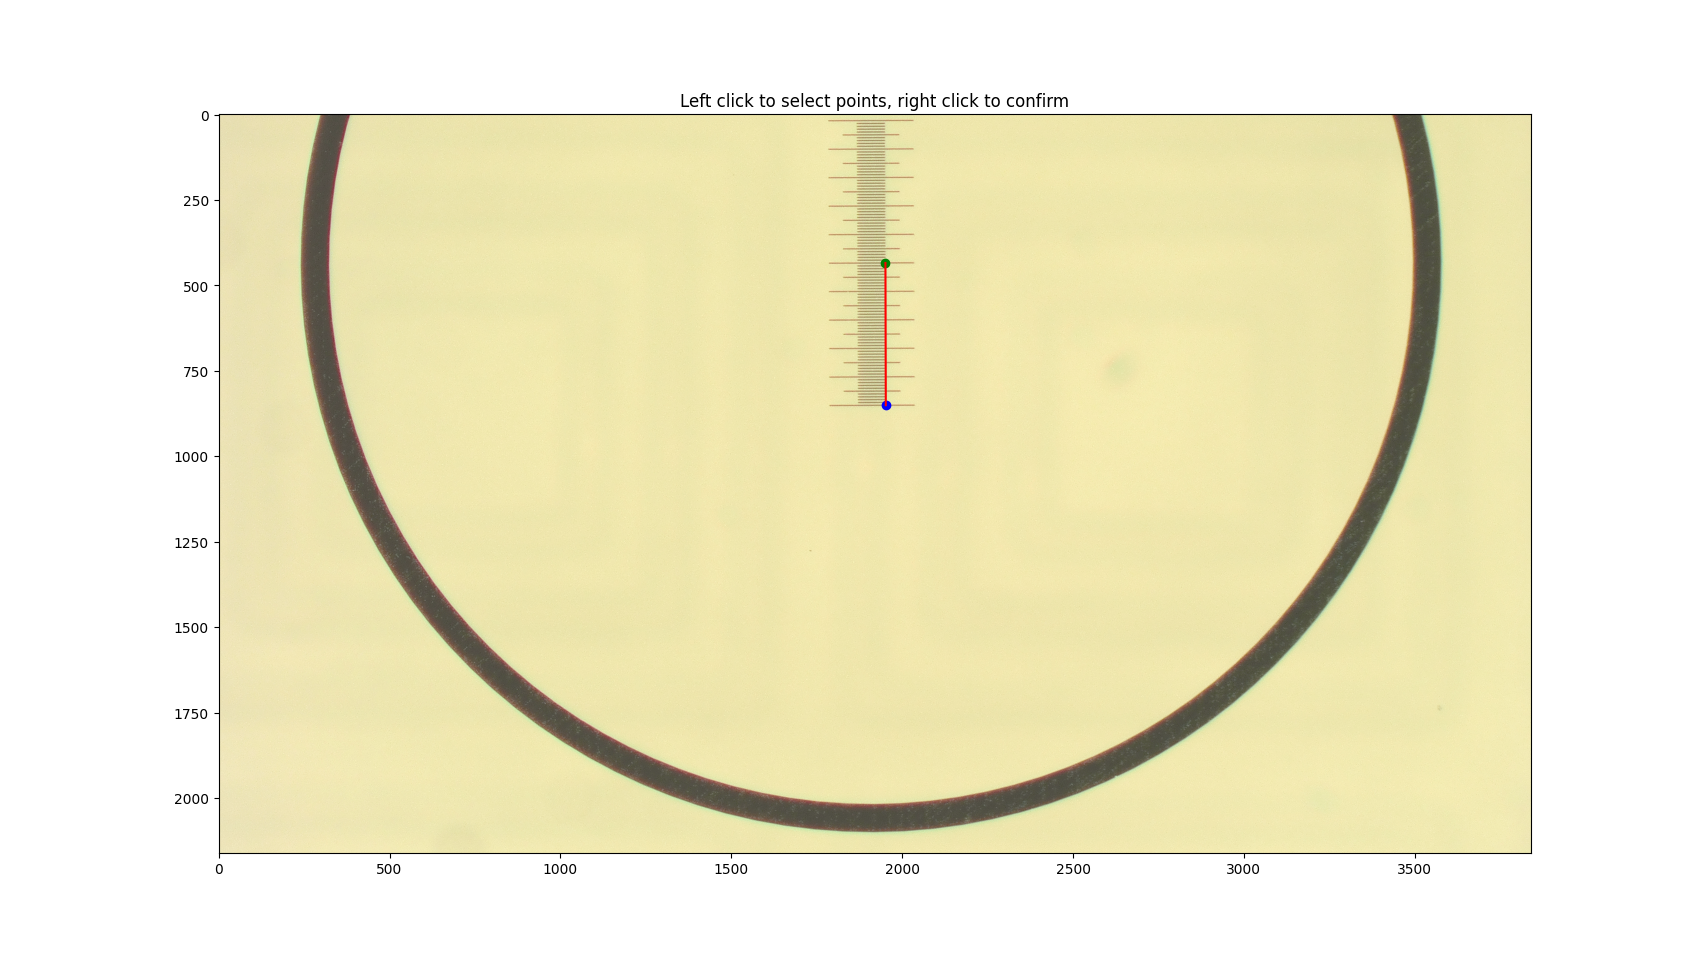
\includegraphics[height=0.5\linewidth]{../diagrams/dpi_measurement_whole.png}
    \caption{Scale Bar for DPI measurements}
    \label{fig:dpi_measurement_whole}
  \end{subfigure}%
  \begin{subfigure}{.5\textwidth}
    \centering
    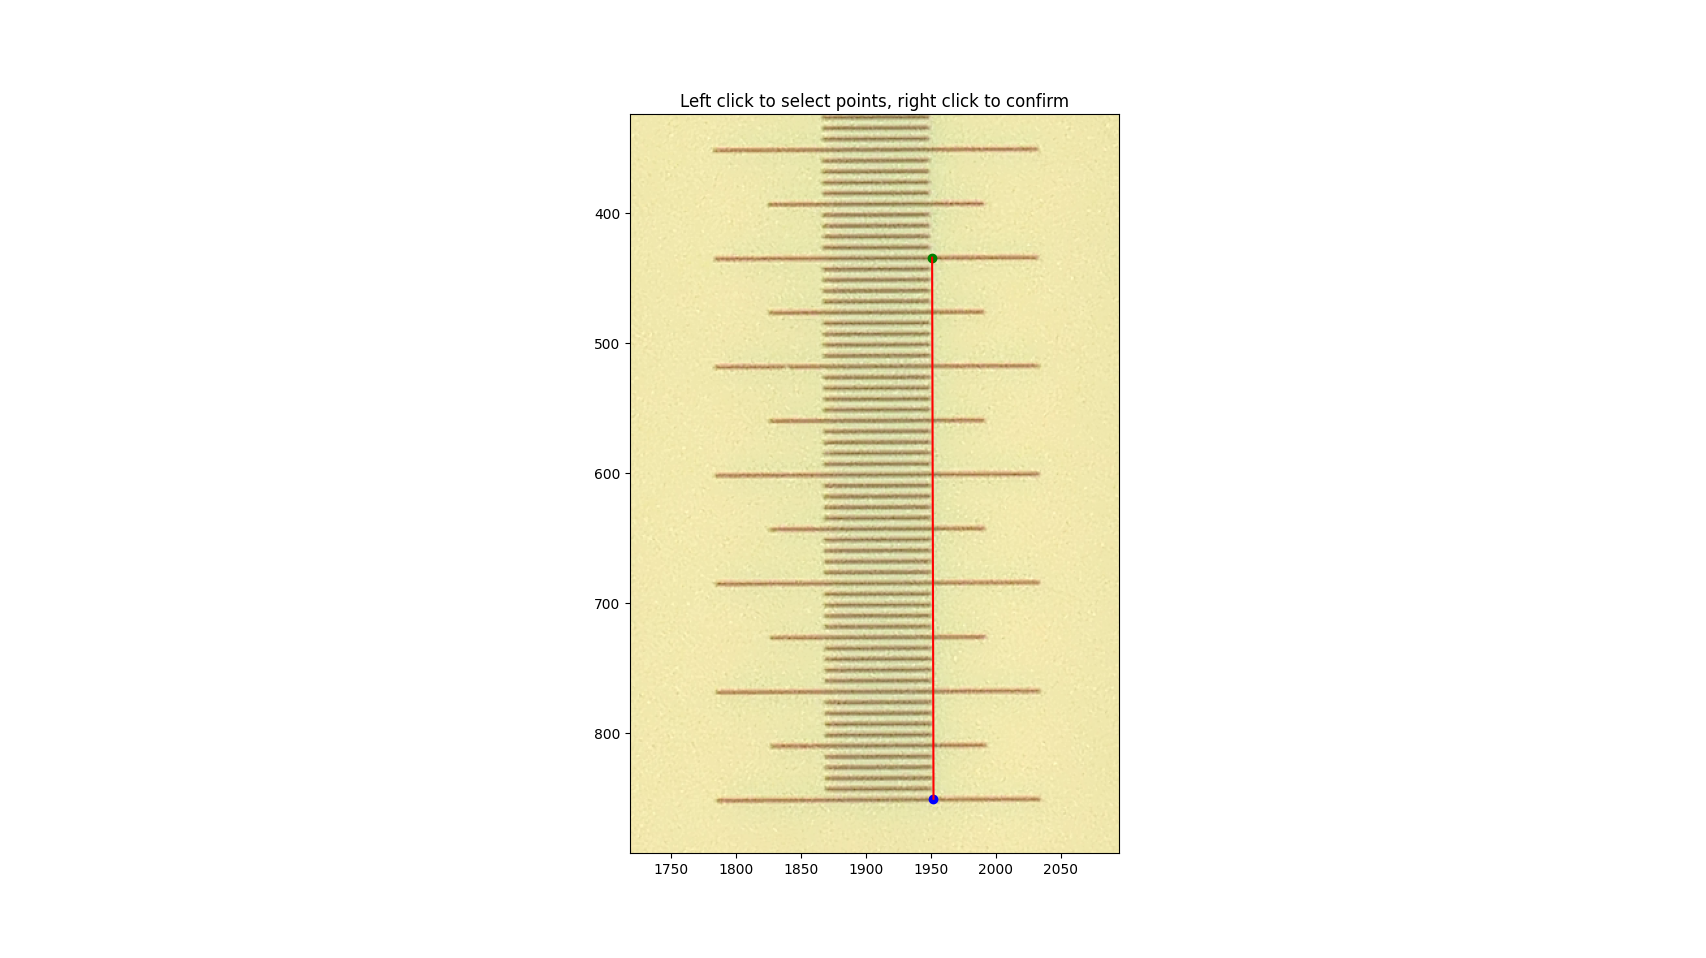
\includegraphics[height=0.5\linewidth]{../diagrams/dpi_measurement_zoomed_2.png}
    \caption{Zoomed in Scale Bar}
    \label{fig:dpi_measurement_zoomed}
  \end{subfigure}
  \caption{Example of a single DPI measurement using a 0.01mm slide scale. The DPI was measured at multiple locations in the field of view both vertically and horizontally. They converged on the same value.}
  \label{fig:dpi_measurements}
\end{figure}

TIM is capable of producing extremely high resolution scans.
A microscopy slide scale with 0.01mm graduations was used to calculate the dots per inch (DPI) of individual images captured from the system (Figure \ref{fig:dpi_measurements}).  
Using this scale we calculated the maximum DPI to be 21,140. This calculation can be replicated using the Python tool we created as necessary for varied lens focal lengths. When downscaling the final stitch, 
DPI scales linearly with the downscale percentage defined in the machine parameters. 

TIM has been used to digitize 90 cookies and is in the process of finishing 1,200 cores. 
Digitizing samples takes significantly longer for cookies than it does for cores (Figure \ref{fig:digitization_time}). This is due to the surface area of cookies requiring more images as their surface area has a square relationship to sample diameter.
For large cookies, the operator can choose to selectively scan a portion of the cookie. Scanning cookies at maximum resolution is unrealistic as the max cookie size is very small. 
To fit into the maximum 2.5 GB limits of a TIFF file, the maximum diameter of a cookie scanned at 30\% of maximum resolution is limited to approximately 130 mm. For cores at maximum resolution, this file size limit 
constrains samples to approximately 1,500 mm in length. Note that a larger ACRO frame would be needed to support this sample length. Samples that are larger than this file size limit are still possible to be scanned but they are no longer stored as a TIFF file. 
An uncompressed binary NumPy memory-mapped array file is produced. This implies that the operator knows how to splice into these files and is comfortable working with NumPy memory-mapped arrays in Python.

\begin{figure}
    \centering
    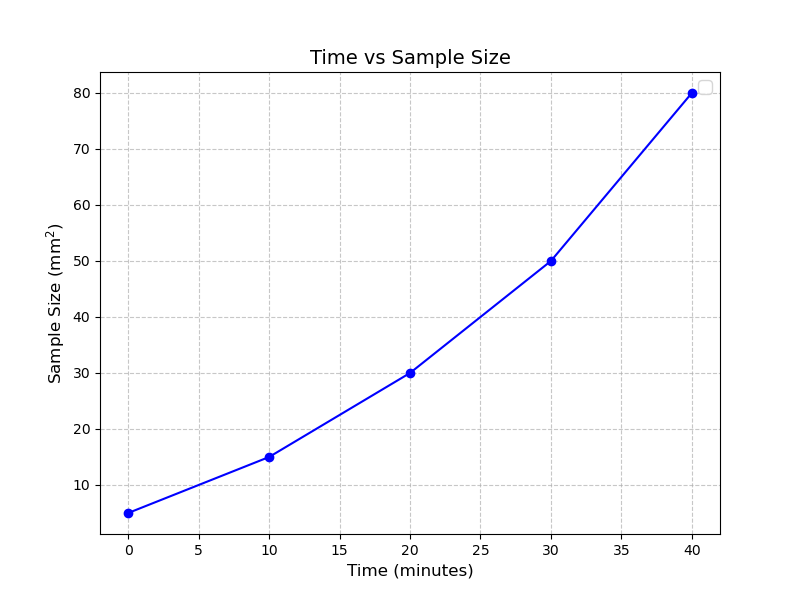
\includegraphics[height=0.5\linewidth]{../../code/plots/time_and_area.png}
    \caption{Time to digitize a sample is dependent on the sample's surface area and the desired final resolution.
    Cores benefit from linear surface area to sample length. The range of sample included are from a 3mm x 220mm core to a 75mm x 56mm cookie. True sampling times are drastically influenced by configurable machine parameters.}
    \label{fig:digitization_time}
\end{figure}

\section{Discussion}
By taking advantage of a common 3 degree of freedom cartesian machine design, powerful edge computing, and a microscope camera we were able to design a cost effective and high resolution digitization tool for wood samples. 
We significantly increased the maximum sample length and maximum resolution compared to common alternatives in the field. 
In addition, the machine design was intended to be readily replicated by labs with minimal engineering experience and equipment. 

\subsection{Strengths and Opportunities}
Our design has tried to minimize the barriers to building this machine in smaller labs. After investing a few hours in the sourcing and assembly of parts, 
the rest of the implementation has been completed. Digitized samples from this machine have been able to have tree rings registered onto their images using CooRecorder.
Integration into a cloud data storage system would be a great addition to remove the need for an operator to move the final data with a physical external drive. 
Further testing with vessel counting models or ring identification models would be an interesting extension to take advantage of high resolution scans.

\bibliographystyle{plainnat}
\bibliography{references}

\end{document}
